\PassOptionsToPackage{dvipsnames}{xcolor}
\documentclass{beamer}

% Frankfurt <3
\usetheme{Frankfurt}

% Some packages
\usepackage{etex}
\usepackage{tikz}
\usepackage{tabularx}
\usepackage{pgfplots} % for tikz
\usepackage{amssymb} % math symbols
\usepackage{pifont} % to get xmark/cmark
\usepackage{booktabs} % commands to better structure tables
\usepackage{xcolor,colortbl} % highlight table rows and columns
\usepackage{graphics} % for resizing

% Tikz options
\usetikzlibrary{calc,trees,positioning,arrows,chains,fit,shapes.geometric,%
    decorations.pathreplacing,decorations.pathmorphing,shapes,%
    matrix,shapes.symbols}

% Other configs and variables
\newcommand{\cmark}{\color{ForestGreen}\ding{52}} % Awesome green check mark
\newcommand{\xmark}{\color{RedOrange}\ding{55}}   % Awesome red cross mark

% Some basic stuff for the first slide
\title{Making recommendations using extremely sparse
       implicit datasets}
\subtitle{SoBazaar Workshop}
\date{2014-06-10}
\author{Martin Christian Havig, Thomas Almenningen \& Herman Schistad}

\begin{document}

  % Title page, showing title, date and authors.
  \begin{frame}
    \titlepage
  \end{frame}

  % Kickstart stuff with e-commerce statistics and competitor overview
  \begin{frame}
    \frametitle{E-commerce in Norway since 2005}
    \begin{figure}[H]
      \centering
      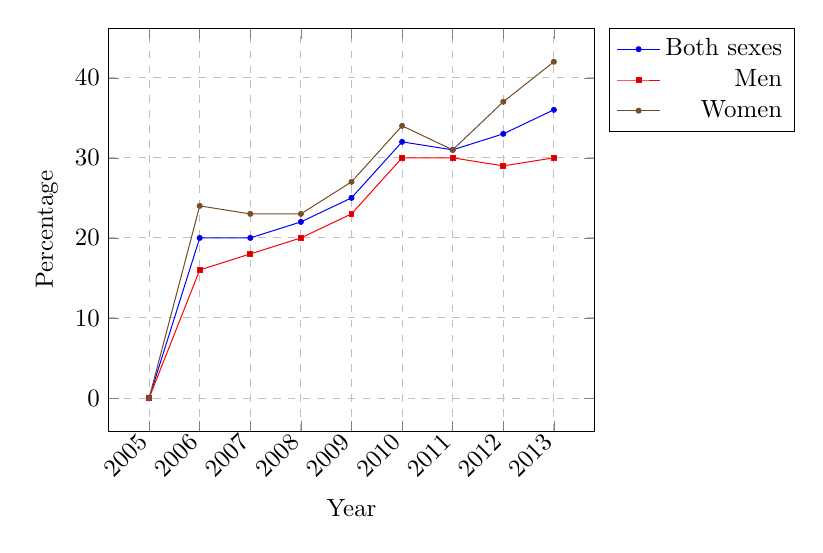
\begin{tikzpicture}[scale=0.9]
        \begin{axis}[
          xlabel={Year},
          ylabel={Percentage},
          legend style={cells={anchor=east}, legend pos=outer north east,},
          xtick=data,
          x tick label style={rotate=45, anchor=east, /pgf/number format/1000 sep=},
          mark size=1.0pt,
          grid=major,
          grid style={dashed},
        ]
        \legend{Both sexes, Men, Women}
        \addplot coordinates {
          (2005, 0)
          (2006, 20)
          (2007, 20)
          (2008, 22)
          (2009, 25)
          (2010, 32)
          (2011, 31)
          (2012, 33)
          (2013, 36)
        };
        \addplot coordinates {
          (2005, 0)
          (2006, 16)
          (2007, 18)
          (2008, 20)
          (2009, 23)
          (2010, 30)
          (2011, 30)
          (2012, 29)
          (2013, 30)
        };
        \addplot coordinates {
          (2005, 0)
          (2006, 24)
          (2007, 23)
          (2008, 23)
          (2009, 27)
          (2010, 34)
          (2011, 31)
          (2012, 37)
          (2013, 42)
        };
        \end{axis}
      \end{tikzpicture}
      \caption{Source: Statistics Norway~\cite{statisticsNorway}}
    \end{figure}
  \end{frame}

  \begin{frame}
    \frametitle{Competitor Overview}
    \framesubtitle{Properties of competitors' recommender systems}
      \begin{table}[H]
          \centering
          \resizebox*{!}{0.6\textheight}{
            \begin{tabular}{lllllll}
                \toprule
                Competitor &
                \multicolumn{1}{l}{\parbox{1.3cm}{ In App \\ Purchase}} &
                \multicolumn{1}{l}{\parbox{1.0cm}{ Most \\ Popular}} &
                \multicolumn{1}{l}{\parbox{1.0cm}{ Similar \\ Items}} &
                \multicolumn{1}{l}{\parbox{1.0cm}{ Want \\ List}} &
                \multicolumn{1}{l}{\parbox{1.9cm}{ Follow \\ Other Users}} &
                \multicolumn{1}{l}{\parbox{2.6cm}{ Personalized \\ Recommendations}} \\ \midrule

                Myntra  & \cmark & \cmark & \cmark & \cmark & \xmark & \xmark \\
                Flink   & \xmark & \cmark & \cmark & \cmark & \cmark & \xmark \\
                Lyst    & \xmark & \cmark & \cmark & \cmark & \cmark & \xmark \\
                Motilo  & \xmark & \cmark & \xmark & \cmark & \cmark & \xmark \\
                Farfetch & \cmark & \cmark & \cmark & \cmark & \xmark & \xmark/\cmark \\
                ModCloth  & \cmark & \cmark & \cmark & \cmark & \xmark & \xmark \\
                UsTrendy  & \cmark & \cmark & \cmark & \cmark & \xmark & \xmark \\
                Polyvore  & \xmark & \cmark & \cmark & \cmark & \cmark & \xmark \\
                Clothia  & \xmark & \cmark & \cmark & \cmark & \cmark & \xmark \\
                Trendabl  & \cmark & \cmark & \cmark & \cmark & \cmark & \xmark \\
                Zalando  & \cmark & \cmark & \cmark & \cmark & \xmark & \xmark \\
                Ellos  & \cmark & \cmark & \cmark & \cmark & \xmark & \xmark \\
                LookBook  & \xmark & \cmark & \cmark & \cmark & \cmark & \xmark \\
                Fahsiolista  & \xmark & \cmark & \xmark & \cmark & \cmark & \xmark \\
                ShopStyle  & \xmark & \xmark & \cmark & \cmark & \xmark & \xmark \\
                MyHabit  & \cmark & \xmark & \cmark & \xmark & \xmark & \xmark \\
                Asos  & \cmark & \cmark & \cmark & \cmark & \cmark & \xmark \\
                Mallzee  & \xmark & \xmark & \xmark & \cmark & \cmark & \cmark \\
                Kwoller  & \xmark & \xmark & \xmark & \cmark & \xmark & \cmark \\
                \bottomrule
            \end{tabular}
          }
      \end{table}
  \end{frame}

  % The table of contents, showing sections and subsections.
  \begin{frame}
    \frametitle{Structure}
    \tableofcontents
  \end{frame}

  % First section concerns the data and general overview of application
  \section{Data analysis and application overview}

  % Some key figures and what they mean.
  \begin{frame}
    \frametitle{SoBazaar Data}
    \framesubtitle{Dataset Summary}
      \begin{table}[H]\centering\resizebox*{!}{0.7\textheight}{\begin{tabular}{l l}\toprule
            Attribute       & Count   \\
            \midrule
            Total number of product events  &    35324 \\
            Unique users ids    &    1532 \\
            Unique item ids     &    5688 \\
            Unique storefronts  &    144 \\
            Unique retailer brands  &    22 \\
            \hline
            Item clicks     &    21400 \\
            Item wants  &    12436 \\
            Item purchases  &    1488 \\
            \hline
            First event & Mon, 07 Oct 2013 10:59:57 GMT \\
            Last event & Mon, 19 May 2014 22:51:19 GMT \\
            Lifetime of data & 224 days \\
            \hline
            Average item click count per user   &    13.968668407310705 \\
            Average item want count per user    &    8.117493472584856 \\
            Average item purchase count per user    &    0.9712793733681462 \\
            \hline
            Average user interaction count per item     &    6.210267229254571 \\
            Average item interaction count per user     &    23.057441253263708 \\
            Median item interaction count per user  &    7.0 \\
    \bottomrule\end{tabular}}\end{table}
  \end{frame}

  % Continuation of key figures w/ visualizations.
  \begin{frame}
    \frametitle{SoBazaar Data}
    \framesubtitle{Cumulative Count of Events on Products}
    \begin{figure}[H]
        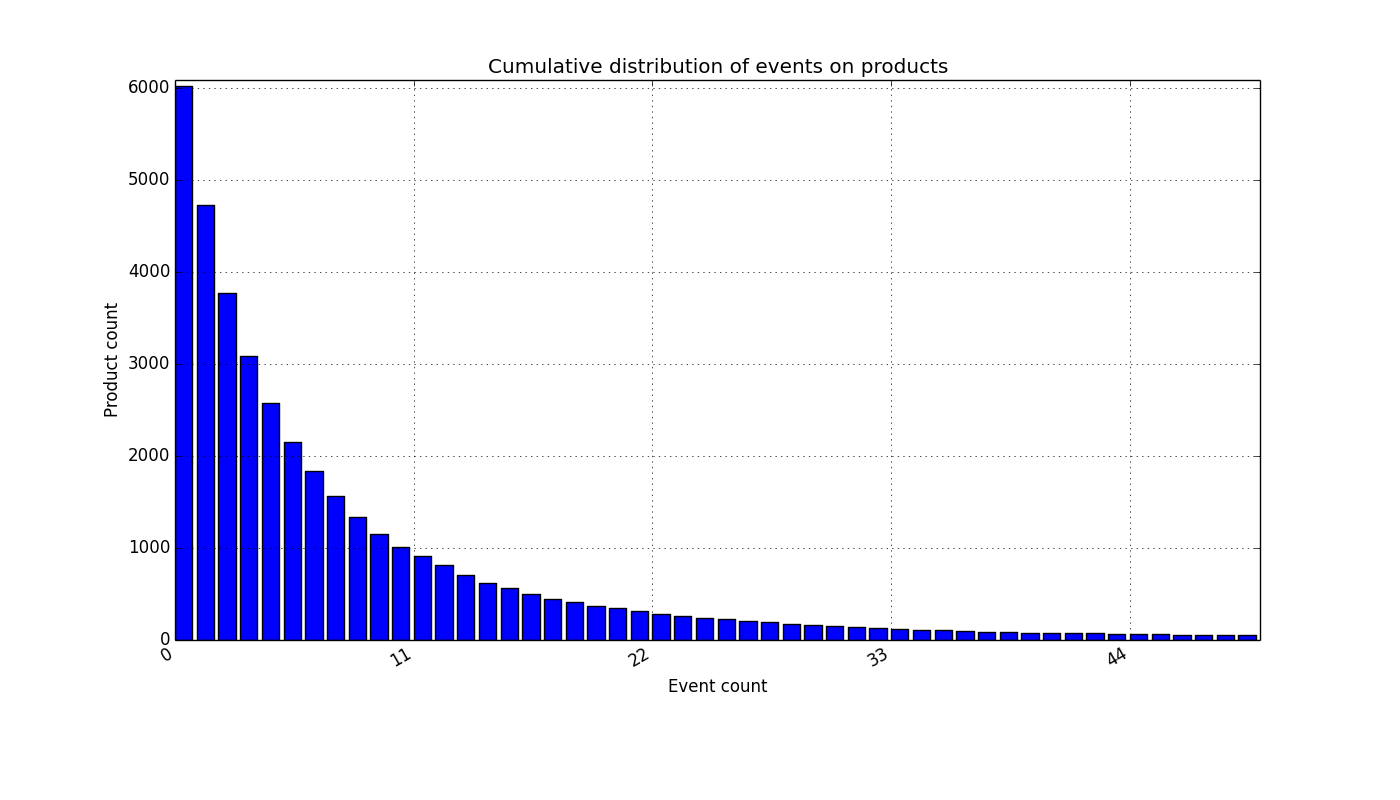
\includegraphics[scale=0.3]{../src/image/product_idcumdistribution.png}
        \centering
    \end{figure}
  \end{frame}

  % Continuation of key figures w/ visualizations.
  \begin{frame}
    \frametitle{SoBazaar Data}
    \framesubtitle{Event Distribution}
    \begin{figure}[H]
        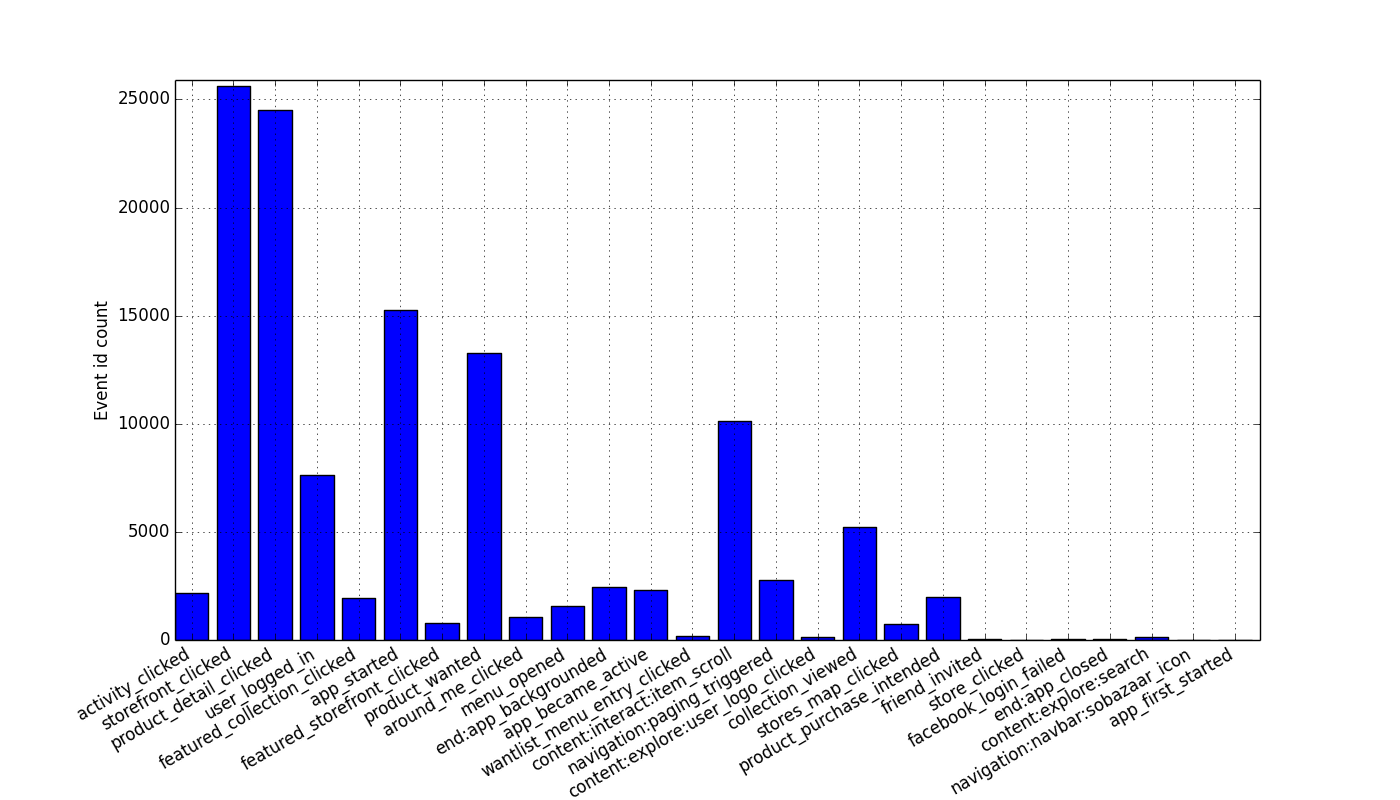
\includegraphics[scale=0.3]{../src/image/event_iddistribution.png}
        \centering
    \end{figure}
  \end{frame}

  \begin{frame}
    \frametitle{SoBazaar Data}
    \framesubtitle{Cumulative Event Distribution Per User}
    \begin{figure}[H]
        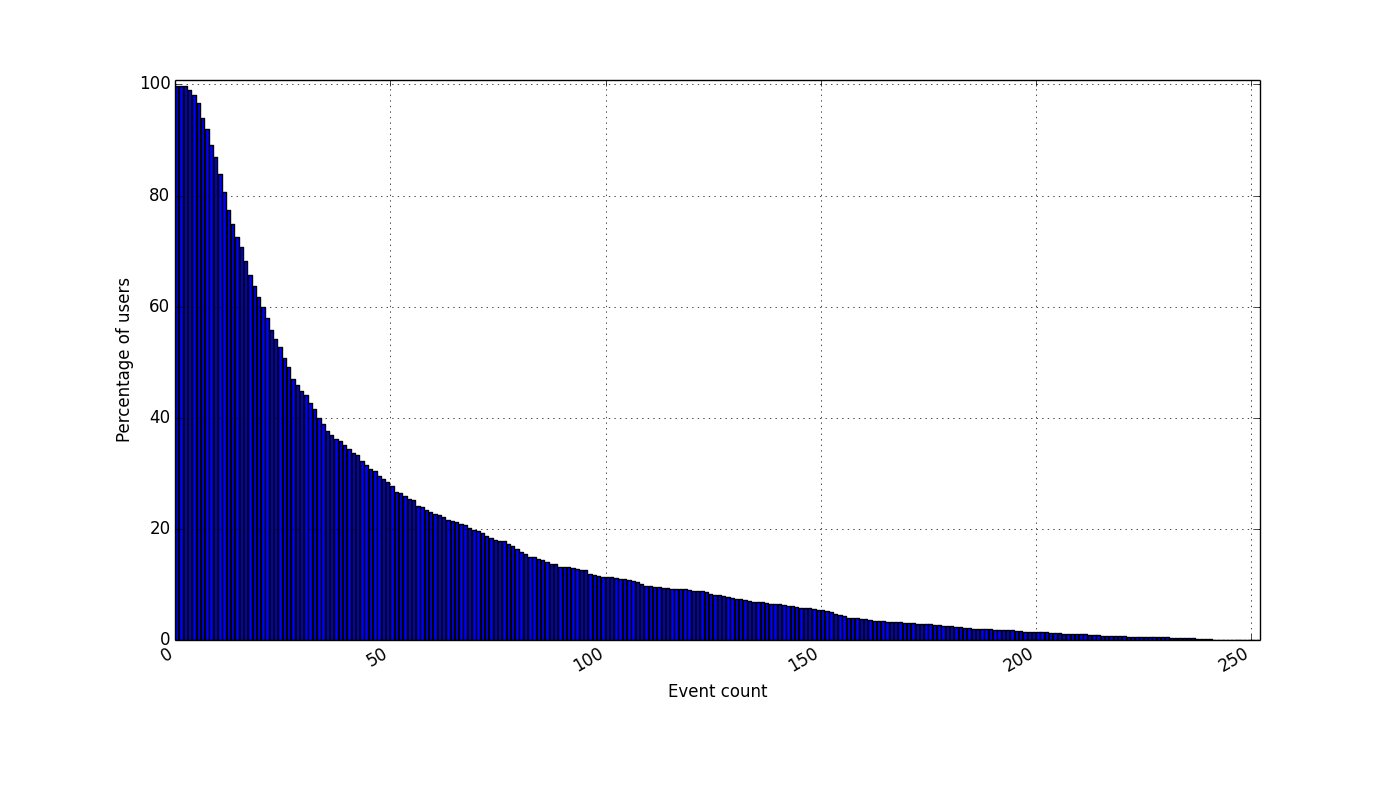
\includegraphics[scale=0.3]{../src/image/user_idcumdistribution.png}
        \centering
    \end{figure}
  \end{frame}

  \begin{frame}
    \frametitle{SoBazaar Data}
    \framesubtitle{Distribution of item account lifetime}
    \begin{figure}[H]
        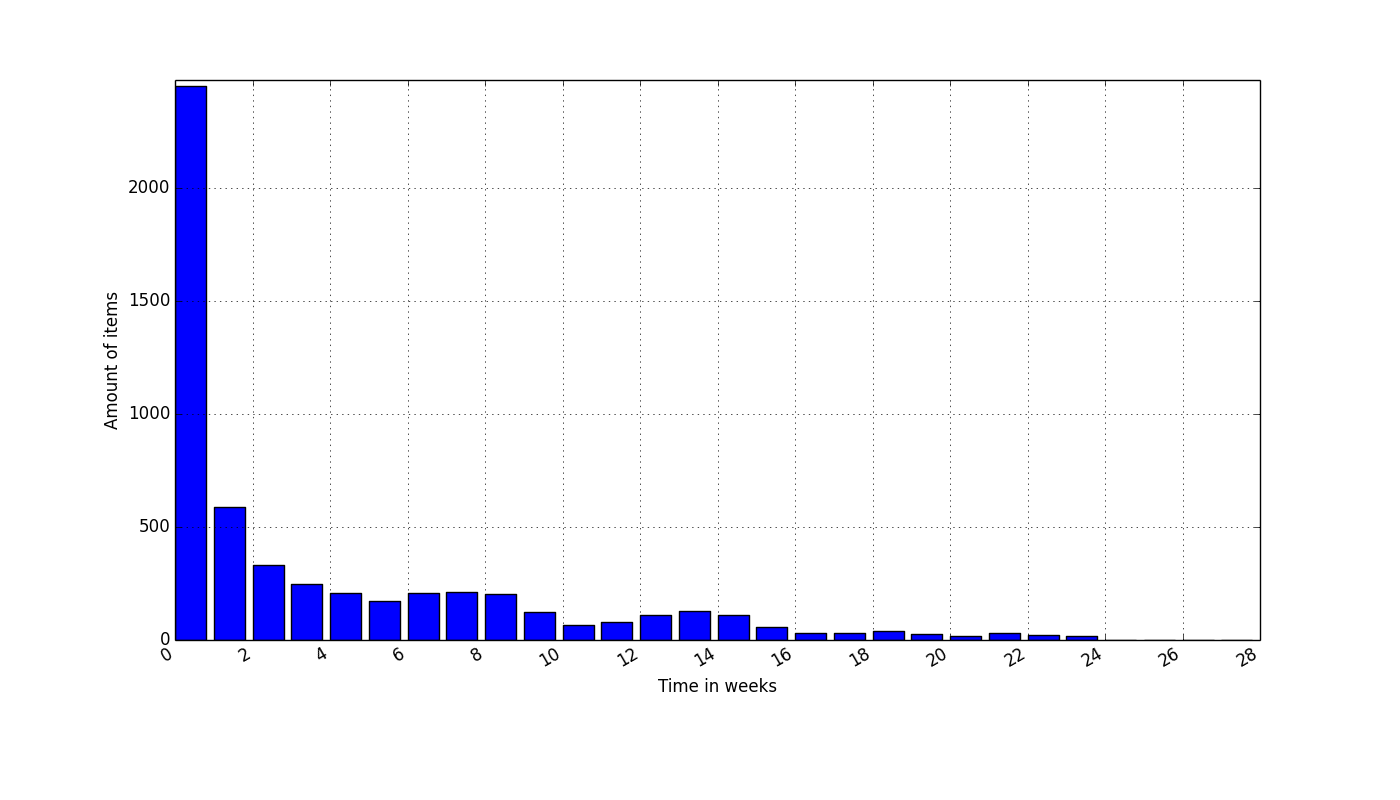
\includegraphics[scale=0.3]{../src/image/itemTimespansdistribution.png}
        \centering
    \end{figure}
  \end{frame}

  % What does it mean that feedback is implicit?
  \begin{frame}
    \frametitle{Implicit feedback}
    \framesubtitle{What is it?}
    \begin{itemize}
      \item Data captured from user behaviour.
      \item Item features and application properties.
      \item Recentness, price, popularity, brand, product properties.
      \item Probabilities of various convertions.
    \end{itemize}
  \end{frame}

  \begin{frame}
    \frametitle{Implicit feedback}
    \framesubtitle{Challenges}
    \begin{itemize}
      \item Not much existing research.
      \item No good evaluation metrics.
      \item No ground truth.
      \item Difficult to weight features.
      \item Performs better in dense environments.
      \item Combining with other sources.
    \end{itemize}
  \end{frame}

  % How we propose to recommend items for SoBazaar
  \begin{frame}
    \frametitle{Application Overview}
    \framesubtitle{Application overview, showing input and output from different
      components in the proposed system}
    \begin{figure}[H]
      \centering
      \resizebox*{!}{0.65\textheight}{
      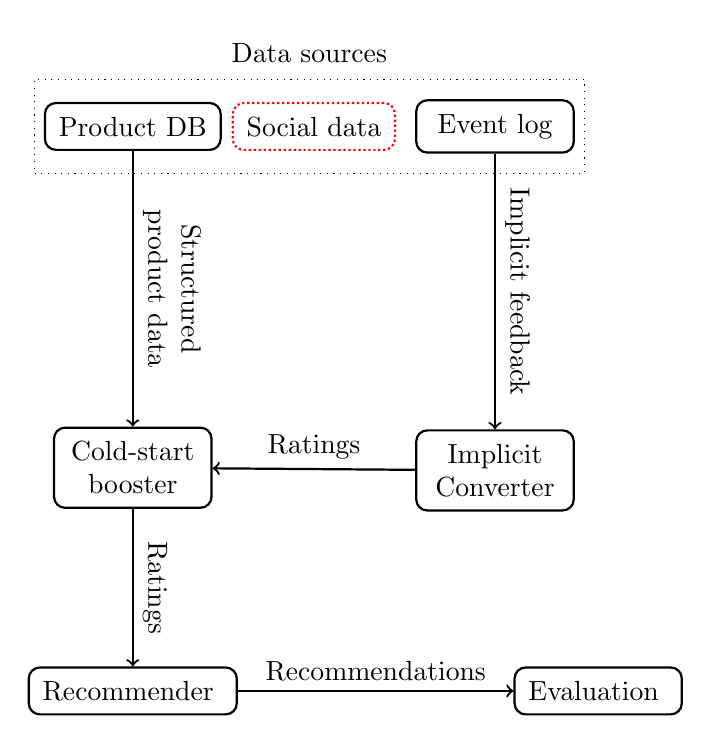
\begin{tikzpicture}[
        % Manually overriden in most of the nodes :-)
        node distance=2.3cm,
        block/.style={
          rectangle,
          draw,
          thick,
          inner sep=5pt,
          align=center,
          rounded corners,
          minimum width=2cm,
        },
        % Special style for the social networks
        social/.style={
          draw=red,
          densely dotted,
        },
        % Box surrounding the data sources.
        dsbox/.style={
          draw,
          dotted,
          minimum height=1.2cm,
        }
      ]

      % Create nodes - first, data sources.
      \node(db)     [block] {Product DB};
      \node(social) [block,social, right of=db] {Social data};
      \node(log)    [block,right of=social] {Event log};

      % Our various 'systems'
      \node(coldstart) [block, below = 3.5cm of db] { Cold-start\\booster };
      \node(converter) [block, below = 3.5cm of log] { Implicit\\Converter };
      \node(recommender) [block, below = 2cm of coldstart] { Recommender };
      \node(evaluation) [block, right = 3.5cm of recommender] { Evaluation };

      % Box around data sources.
      \node (datasources) [dsbox, fit=(db) (social) (log)] {};
      \node at (datasources.north) [above, inner sep=2mm] {Data sources};

      % Draw the links between systems and data sources.
      \path[->,thick]
         (log) edge [] node [sloped, above] {Implicit feedback} (converter)
         (db) edge [] node [sloped, above, text width=3cm, align=center] {Structured\\product data} (coldstart)
         (converter) edge [] node [sloped, above] {Ratings} (coldstart)
         (coldstart) edge [] node [sloped, above] {Ratings} (recommender)
         (recommender) edge [] node [sloped, above] {Recommendations} (evaluation);

      \end{tikzpicture}
      }
    \end{figure}
  \end{frame}

  % Second section, going through each of these components.
  \section{Proposed system components}

  % Component one: creating implicit ratings.
  \begin{frame}
    \frametitle{Converting Implicit Feedback}
    \begin{itemize}
      \item We looked at \textit{price}, \textit{item popularity} and
      \textit{recentness}.
      \item What is recentness? Both number of days and ordering of events.
      \item Base our methods on probability of an event happening and then
      penalize based on said features.
    \end{itemize}
  \end{frame}

  \begin{frame}
    \frametitle{Converted Implicit Feedback}
    \framesubtitle{Distribution using blend of ordering and number of days since event, with logistic and linear penalization functions, overlayed with density function}
    \begin{figure}[H]
        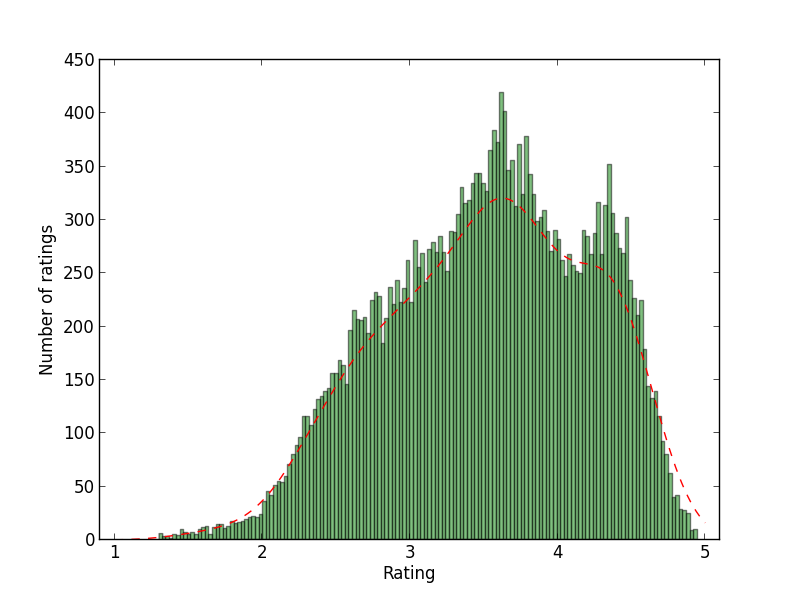
\includegraphics[scale=0.4]{../src/image/dist-blend-price-popularity-recentness}
        \centering
    \end{figure}
  \end{frame}

  % Component two: filterbots and cold-start stuff.
  \begin{frame}
    \frametitle{Cold start boosting}
    \begin{itemize}
      \item Important when we have few users and sparse datasets.
      \item Also important for handling new users and items.
      \item Filterbots are used in thesis, in order to simulate user behaviour.
      \item Can extend with social, demographic and content-based data.
      \item Includes switching between recommender methods. Use naive methods
      for cold-start users.
    \end{itemize}
  \end{frame}

  % Component three: actually making recommendations.
  \begin{frame}
    \frametitle{Making recommendations}
    \begin{itemize}
      \item Implicit ratings requires us to look at methods differently.
      \item Methods used: \textit{itembased}, \textit{userbased}, \textit{most
      popular}, \textit{random}, \textit{SVD}, \dots
      \item Best results with matrix factorization.
      \item We do not perform any dynamic switching.
    \end{itemize}
  \end{frame}

  % Component four: how to evaluate the results.
  \begin{frame}
    \frametitle{Evaluation}
    \begin{itemize}
      \item Recap: Evaluating implicit feedback is difficult. You have no
      \textit{ground truth}.
      \item Best way of confirming performance: online experiments.
      \item Various ways of splitting dataset.
      \item Perform user studies to understand underlying features and
      accuracy.
    \end{itemize}
  \end{frame}

  \begin{frame}
    \frametitle{Evaluation How}
    \framesubtitle{Comparing Ratings}
    \begin{figure}[H]
        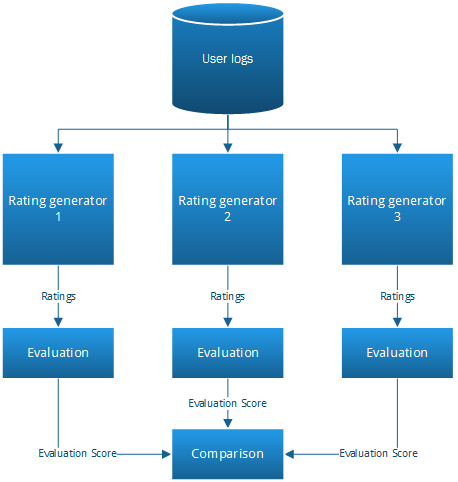
\includegraphics[scale=0.4]{../src/image/ratinggeneval.png}
        \centering
    \end{figure}
  \end{frame}

  \begin{frame}
    \frametitle{Evaluation How}
    \framesubtitle{Overview of how the generated ratings from the implicit feedback can be evaluated}
      \begin{figure}
      \centering
      \resizebox*{!}{0.5\textheight}{

          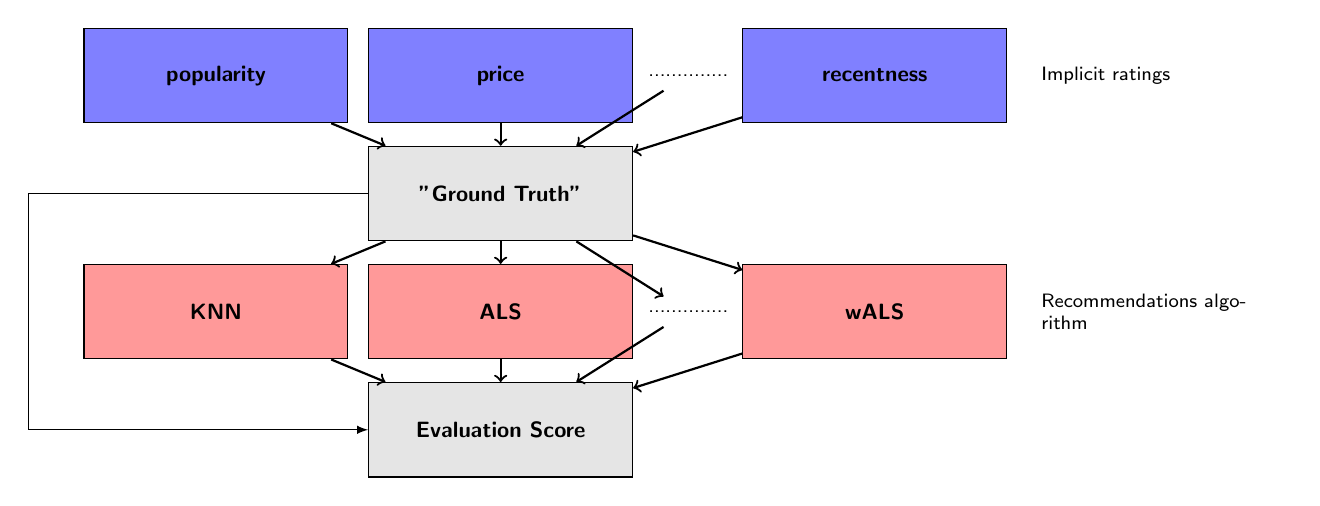
\begin{tikzpicture}
          [node distance = 1cm, auto,font=\footnotesize,
          % STYLES
          every node/.style={node distance=1.5cm},
          % The comment style is used to describe the characteristics of each process
          comment/.style={rectangle,
                          inner sep= 5pt,
                          text width=3cm,
                          node distance=0.25cm,
                          font=\scriptsize\sffamily},
          % small comment lol
          comment-small/.style={rectangle,
                                inner sep= 5pt,
                                text width=1cm,
                                node distance=0.25cm,
                                font=\scriptsize\sffamily},
          % The nonProcess style
          nonProcess/.style={rectangle,
                             draw,
                             inner sep=5pt,
                             text width=3cm,
                             text badly centered,
                             minimum height=1.2cm,
                             font=\footnotesize\sffamily},
          % The process style is used to draw the processs' name
          process/.style={rectangle,
                          draw,
                          fill=black!10,
                          inner sep=5pt,
                          text width=3cm,
                          text badly centered,
                          minimum height=1.2cm,
                          font=\bfseries\footnotesize\sffamily},
          % ratingsGenerator style
          ratingsGenerators/.style={rectangle,
                                    draw,
                                    fill=blue!50,
                                    inner sep=5pt,
                                    text width=3cm,
                                    text badly centered,
                                    minimum height=1.2cm,
                                    font=\bfseries\footnotesize\sffamily},
          % racommendation algorithms
          recAlgs/.style={rectangle, draw, fill=red!40, inner sep=5pt, text width=3cm, text badly centered, minimum height=1.2cm, font=\bfseries\footnotesize\sffamily}]

          % Draw processs
          \node [ratingsGenerators] (rg1) {popularity};
          \node [ratingsGenerators, right=0.25 of rg1] (rg2) {price};
          \node [comment-small, right=0.01 of rg2] (dotdotdot) {..............};
          \node [ratingsGenerators, right=0.01 of dotdotdot] (rg3) {recentness};
          \node [process, below of=rg2] (gt) {"Ground Truth"};
          \node [recAlgs, below of=gt] (ra2) {ALS};
          \node [recAlgs, left=0.25 of ra2] (ra1) {KNN};
          \node [comment-small, right=0.01 of ra2] (dotdotdot2) {..............};
          \node [recAlgs, right=0.01 of dotdotdot2] (ra3) {wALS};
          \node [process, below of=ra2] (eval) {Evaluation Score};
          \node [comment, right=0.25 of rg3] (comment-rg3) {
            Implicit ratings
          };
          \node [comment, right=0.25 of ra3] (comment-ra3) {
            Recommendations algorithm
          };
          % Draw the links between processs
          \path[->,thick]
            (rg1) edge (gt)
            (rg2) edge (gt)
            (dotdotdot) edge (gt)
            (rg3) edge (gt)
            (gt) edge (ra1)
            (gt) edge (ra2)
            (gt) edge (dotdotdot2)
            (gt) edge (ra3)
            (ra1) edge (eval)
            (ra2) edge (eval)
            (dotdotdot2) edge (eval)
            (ra3) edge (eval);
          \draw[>=latex,->] (gt) -- +(-6,0) |- (eval);
          \end{tikzpicture}
          }
        \end{figure}
  \end{frame}


  % Section three: a summary and conclusions from our work.
  \section{Results and future work}

  % Some thoughts on what we have found.
  \begin{frame}
    \frametitle{Conclusions}
    \begin{itemize}
      \item Our proposed system improves results compared to all binary
      recommenders.
      \item Matrix-factorizations proves to yield best results, although no
      dynamic switching is performed.
      \item The implicit ratings generated by a blend of price, popularity and
      recentness consistently gives best results.
      \item Weak item features yields no distinct gain in precision.
    \end{itemize}
  \end{frame}

  % Figure showing system in relation to "the sky".
  \begin{frame}
    \frametitle{How to implement in SoBazaar}
    \framesubtitle{High level proposal of cloud based recommender}
    \begin{figure}[H]
        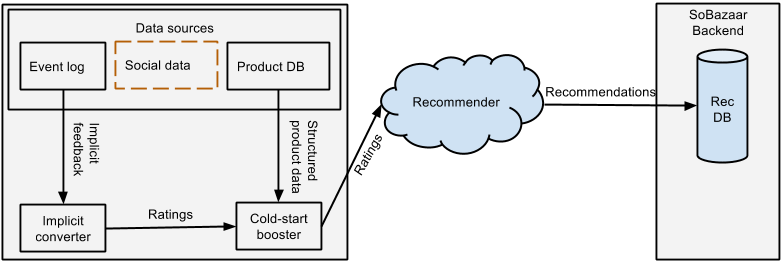
\includegraphics[scale=0.4]{../src/image/theCloud}
        \centering
    \end{figure}
  \end{frame}

  % How can future results be improved?
  \begin{frame}
    \frametitle{Improving results}
    \begin{itemize}
      \item Add ways to provide negative feedback.
      \item Include social and demographic data.
      \item Use simple demographic-based methods on new users, increase
      complexity in accordance to density.
      \item Kick-start recommendations by asking for preferences.
      \item Better results can be achieved with using Tinder-like interface.
      \item Ensure that a framework for online evaluation, is in place.
    \end{itemize}
  \end{frame}

  \begin{frame}[allowframebreaks]
    \frametitle{References}
    \bibliographystyle{plain}
    \bibliography{../src/references}
  \end{frame}

  \begin{frame}
    \huge Our largest gratitude to all of you!
  \end{frame}

\end{document}
